\chapter{Appendix: Resonator Fitting\label{ch:AppA}}

As discussed in Ch. \ref{ch:4_3DGKP}, a large part of the experimental work in this thesis involved probing 3D cavity resonators using classical microwave fields --- either to characterize the intrinsic properties (such as resonator internal and coupling losses) or, for the case of our 3D cavity-fluxonium device, to readout the state of the qubit and more broadly interact with the rest of the system. In this appendix, we will briefly derive from first principles the resonance lineshape of a single-mode resonator coupled to a readout transmission line in a so-called reflection configuration. This simple example can be treated theoretically using the input-output formalism, yet is general enough to cover all of the experiments performed in this thesis. 

We start by considering a linear resonator mode $\hat{a}$ with angular frequency $\omega_0$ coupled to a transmission line. The Hamiltonian describing this mode is that of a quantum harmonic oscillator, $\hat{H} = \h\omega_0 \hat{a}^\dagger \hat{a}$. Without the transmission line, the dynamics of $\hat{a}$ are given in the Heisenberg picture by $\partial_t\hat{a} = -i[\hat{a}, \hat{H}] = -i\omega_0\hat{a}$, leading to the familiar oscillatory motion of $\hat{a}(t)$ in the oscillator's phase space. However, if we include losses and coupling to the transmission line, the dynamics are modified in the form of a Heisenberg-Langevin equation \cite{walls1994quantum, gardiner2004quantum, clerk2010introduction}:
\begin{equation}
    \odv*{\hat{a}}{t}(t) = -i\omega_0\hat{a} - \Big(\frac{\kappa_c + \kappa_i}{2}\Big)\hat{a} + \sqrt{\kappa_c}\hat{a}_{\rm in}(t)
    \label{eq:A_heisenberg}
\end{equation}
Here, we include a damping term proportional to the total loss rate $\kappa = \kappa_c + \kappa_i$, where $\kappa_i$ is the \textit{intrinsic loss} of the mode due to uncontrolled interaction with environmental degrees of freedom and $\kappa_c$ is the \textit{coupling loss} to the transmission line (which we as experimenters may control for in design)\footnote{For a full derivation of this Heisenberg-Langevin equation in the context of superconducting circuits, two great expository references are the PhD theses of Audrey Bienfait \cite{bienfait2016thesis} and Steven Touzard \cite{touzard2019thesis}.}. As an example of a setup that implements Eq. \eqref{eq:A_heisenberg}, we may refer back to Fig. \ref{fig:4-3DGKP-schematic-2}(d) of the main text, which shows a schematic of our 3D experiment and, in particular, a model of the cavity resonators. There, the coupling $\kappa_c$ is implemented via a physical pin sticking into the cavity whose length (or rather, distance from the cavity post) determines the coupling strength \cite{axline2016architecture}. The pin is connected to a microwave drive line, which gives rise to the source term $\sqrt{\kappa_c}\hat{a}_{\rm in}(t)$ in Eq. \eqref{eq:A_heisenberg} in terms of the input propagating field $\hat{a}_{\rm in}$ (travelling to the cavity) in the transmission line. We can also have a transmission line field propagating away from the cavity, which we call $\hat{a}_{\rm out}$. 

In circuit QED experiments, we typically interact with readout resonators using a classical field $\alpha_{\rm in}(t)$ associated with a coherent state $\ket{\alpha_{\rm in}}$ in the input transmission line, resulting in a large intra-resonator field $\alpha(t) = \ev{\hat{a}}(t)$. Taking the expectation values on both sides of Eq. \eqref{eq:A_heisenberg}, we thus get $\partial_t \alpha(t) = -i\omega_0\alpha - (\kappa_c + \kappa_i)\alpha/2 + \sqrt{\kappa_c}\alpha_{\rm in}(t)$. Note that by defining a drive amplitude $\epsilon(t) = i\sqrt{\kappa_c}\alpha_{\rm in}(t)$, we can now self-consistently interpret the source term as coming from a Hamiltonian drive $\epsilon(t)(\hat{a} + \hat{a}^\dagger)$ on the system, which also motivates the discussion presented in Sec. \ref{sec:2_control_nonlinearity_drive}. 

If we take a Fourier transform $\mathcal{F}[\bullet]$ of the above equation, we can calculate\footnote{Recalling the definition $\mathcal{F}[\alpha(t)] \equiv \int \alpha(t) e^{i\omega t}dt$, we can derive $\mathcal{F}[\partial_t\alpha(t)] = -i\omega \alpha(\omega)$ via integration by parts.} the frequency domain response:
\begin{equation}
    \alpha(\omega) = \frac{2\sqrt{\kappa_c}}{\kappa_c + \kappa_i - 2i(\omega-\omega_0)} \alpha_{\rm in}(\omega)
    \label{eq:inputoutput-freq-domain}
\end{equation}
This equation gives us the ability to calibrate the mean circulating photon number $\bar{n} = |\alpha|^2$ in the resonator, in terms of the input power $P_{\rm in} = \myhbar\omega |\alpha_{\rm in}|^2$ seen by the device. Specifically, on resonance ($\omega = \omega_0$), we get:
\begin{equation}
    \bar{n} = \frac{4\kappa_c P_{\rm in}}{\myhbar\omega_0(\kappa_c + \kappa_i)^2}
\end{equation}
In the limit $\kappa_i \ll \kappa_c$ that we take for readout, this reduces to $P_{\rm in} = \kappa_c\myhbar\omega_0 \bar{n}/4$. 

\noindent Now, the classical continuity equation for the propagating fields gives rise to the so-called \textit{input-output relation} \cite{clerk2010introduction}, which expresses the resonator mode $\hat{a}$ in terms of the transmission line fields: 
\begin{equation}
    \hat{a}_{\rm in}(t) + \hat{a}_{\rm out}(t) = \sqrt{\kappa_c} \hat{a}(t)
    \label{eq:inputoutput}
\end{equation}
In combination with Eq. \eqref{eq:inputoutput-freq-domain}, this relation allows us to express the reflected coherent output signal $\alpha_{\rm out}(\omega)$ in terms of the input signal $\alpha_{\rm in}(\omega)$ sent in to the resonator. In particular, their ratio defines
\begin{equation}
   S_{11}(\omega) = \frac{\alpha_{\rm out}(\omega)}{\alpha_{\rm in}(\omega)} = \frac{\kappa_c - \kappa_i + 2i(\omega - \omega_0)}{\kappa_c + \kappa_i - 2i(\omega - \omega_0)},
   \label{eq:A_S11_ideal}
\end{equation}
i.e., a reflection coefficient. It tells us the amplitude/phase response of the received output signal  $\alpha_{\rm out}$ in terms of the incident field $\alpha_{\rm in}$ we apply. Note, the choice to call this coefficient ``$S_{11}$'' can be traced back to the S-matrix formalism \cite{kurokawa1965power, gardiner1985input}, which extends the analysis here to multi-port devices, and defines $S_{ij}(\omega) = \alpha_{{\rm out}, i}(\omega)/\alpha_{{\rm in}, j}(\omega)$. We get the same expression if we analyze this setup from an electrical engineering perspective using transmission line theory. In our case, however, we consider just a single-port device, i.e., a cavity resonator in reflection configuration, and so the single S-parameter for the reflected signal is given by $S_{11}(\omega)$; this is also what we measure experimentally using a Vector Network Analyzer (VNA) in the lab.  

In practice, the abstract picture of a transmission line here needs to be physically realized in our microwave setup. Our specific readout setup is shown in Fig. \ref{fig:4-microwave-wiring-diagram}. It is worth noting that we used a (3-port) device called a microwave circulator to implement the ``reflection'' measurement of the cavity in an otherwise ``transmission''-like setup. For a measurement on the VNA, we simply connect its ports to the input and output lines, and the measured response indeed should follow Eq. \eqref{eq:A_S11_ideal}. Of course, there are certain experimental factors that need to be accounted for. These include (i) losses in the microwave cables; (ii) a phase offset of the initial input signal; and (iii) the \textit{propagation delay} (the time it takes for a signal to reach the cavity and return back due to the physical distance between the VNA and the cavity). Also known as the \textit{electrical delay}, this last factor causes the output signal phase to vary with frequency based on the speed of light in the microwave cables. To account for all of these effects, we typically fit experimental data to a modified response function that is given by:
\begin{equation}
   S_{11}^{\rm exp}(\omega) = Ae^{i\phi} e^{2\pi i\lambda\omega} \times \bigg[\frac{\kappa_c - \kappa_i + 2i(\omega - \omega_0)}{\kappa_c + \kappa_i - 2i(\omega - \omega_0)}\bigg]
\end{equation}
where $A$ is an amplitude, $\phi$ is a phase offset, and $\lambda$ encodes the electrical delay. 





Finally, we sometimes also see other experimental non-idealities in a realistic microwave setup such as impedance mismatches in the lines \cite{probst2015efficient} or imperfections in the circulator \cite{rieger2023fano}. These effects can lead to a so-called \textit{Fano resonance} of the cavity, resulting in an asymmetric lineshape of the magnitude response $|S_{11}(\omega)|$. To account for this, we thus typically further modify the fit function to have a complex-valued coupling constant $\kappa_e = |\kappa_e|e^{i\varphi_0}$ \cite{probst2015efficient}. The total linewidth $\kappa$ of the cavity is then defined  in terms of the real part of this coupling constant, $\kappa = \kappa_i + {\rm Re}(\kappa_e)$, and the $S_{11}$ response is given in terms of the full complex-valued $\kappa_e$ via:
\begin{equation}
    S_{11}^{\rm fano}(\omega) = \frac{2i(\omega-\omega_0) + \kappa -  2{\rm Re}(\kappa_e)(1+i\tan(\varphi_0))}{2i(\omega-\omega_0) + \kappa}
    \label{eq:A_S11_fano}
\end{equation}
We used this Fano-corrected fit function when analyzing some of our cavity responses. In particular, following up from a comment made in Ch. \ref{ch:4_3DGKP}, we used this for determining the quality factors $Q_i = \omega_0/\kappa_i$ of our 3D cavity resonators. An example of such a response for our bare ``Mark II'' cavity storage resonator (i.e., without the fluxonium chips inserted) is plotted below, from which we extract the characteristic lifetime $T_1 = 1/\kappa_i \approx 765$ $\mu$s. 
\begin{figure}[h]
    \centering
    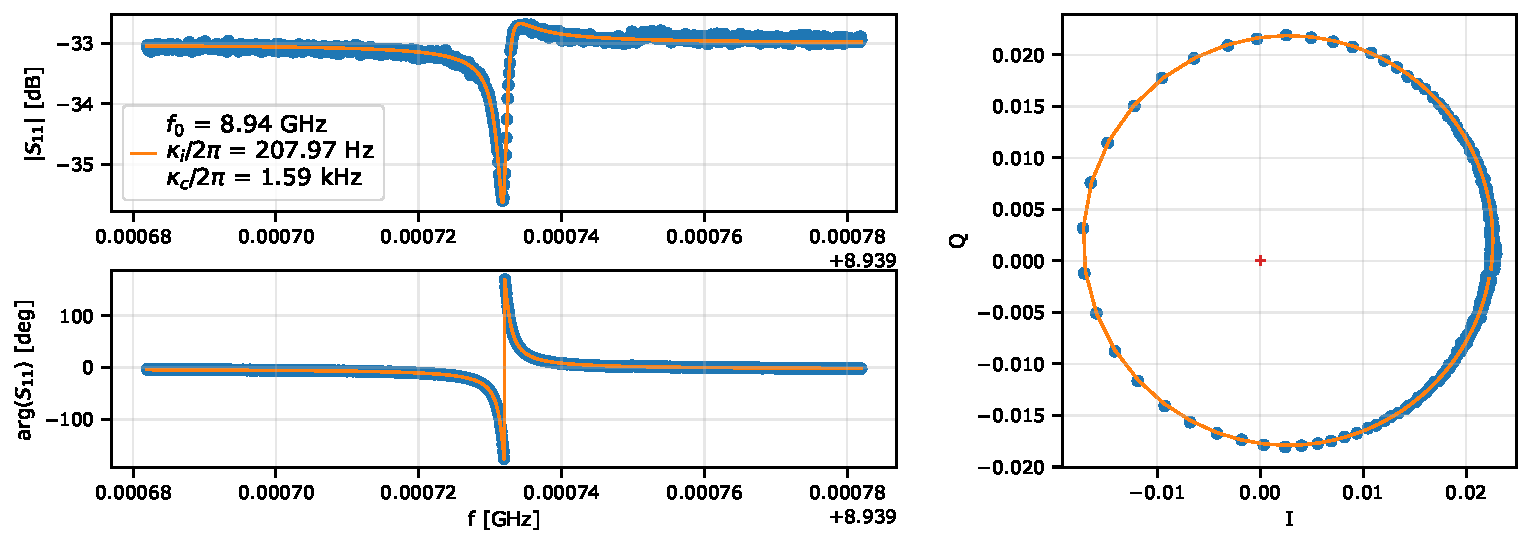
\includegraphics[width=\linewidth]{Figures/A/Storage_Res_S11_Fit.pdf}
    \caption{$S_{11}$ magnitude and phase response of our Mark II storage cavity plotted vs. frequency $f = \omega/2\pi$. From a fit to Eq. \eqref{eq:A_S11_fano}, we extract the resonator frequency $f_0 = \omega_0/2\pi$ and the internal and coupling losses $\kappa_i$ and $\kappa_c \equiv {\rm Re}(\kappa_e)$. The internal loss determines the intrinsic quality of the resonator, from which we can extract a lifetime $T_1 = 1/\kappa_i \approx 765$ $\mu$s.}
    \label{fig:A_Storage_Res_S11_Fit}
\end{figure}